\documentclass[pdftex]{beamer}
%\documentclass[notes=show]{beamer}
%\documentclass[xcolor=dvipsnames]{beamer}

\usepackage{amssymb}
\usepackage{latexsym}
\usepackage{amsfonts}
\usepackage{amsmath}
\usepackage[absolute,overlay]{textpos}
\usepackage[english]{babel}
\usepackage[latin1]{inputenc}
%\usepackage{times}
\usepackage[T1]{fontenc}
\usepackage{tabularx}
\newcolumntype{Y}{>{\small\raggedright\arraybackslash}X}
\usepackage{graphicx}
\usepackage{bigstrut}
\usepackage{bbm}
\usepackage{mathrsfs}
\usepackage{epsfig}
\usepackage{array}
%\usepackage{natbib}

\mode<presentation> {
%\usetheme[left,width=1.7cm]{Berkeley}
%\usetheme{default}
\usetheme{Boadilla}
  \usecolortheme[RGB={103,102,204}]{structure}
%\usecolortheme{dove}
  \useoutertheme{infolines}
  \setbeamercovered{transparent}
 }

%\renewcommand{\familydefault}{cmss}
%\renewcommand{\mathrm}{\mathsf}
%\renewcommand{\textrm}{\textsf}
\usefonttheme{serif}
\newcommand{\X}{{\mathbf{X}}}
\newcommand{\x}{{\mathbf{x}}}
\newcommand{\E}{\mathsf{E}}
\newcommand{\V}{\mathsf{Var}}

\DeclareGraphicsExtensions{.jpg,.pdf,.mps,.png}

    %%%%%%%%%%%%%%%%%%%%%%%%%%%%%%%%%%%%%%%%%%%%%%%%%%%%%%%%%%%%%%%%%%%%%%%%%%%%%%
    %         Neue Kommandos f�r fette Mathebuchstaben innerhalb von Formeln     %
    %%%%%%%%%%%%%%%%%%%%%%%%%%%%%%%%%%%%%%%%%%%%%%%%%%%%%%%%%%%%%%%%%%%%%%%%%%%%%%
    \newcommand{\bom}{\boldmath}
    \newcommand{\ubom}{\unboldmath}
    \newcommand{\mb}{\mathbf}

    \newcommand{\fmalpha}{\mbox{\bom${\alpha}$}}               %Fettes alpha
    \newcommand{\fmbeta}{\mbox{\bom${\beta}$}}                 %Fettes beta
    \newcommand{\fmgamma}{\mbox{\bom${\gamma}$}}               %Fettes gamma
    \newcommand{\fmdelta}{\mbox{\bom${\delta}$}}               %Fettes delta
    \newcommand{\fmepsilon}{\mbox{\bom${\epsilon}$}}           %Fettes epsilon
    \newcommand{\fmvarepsilon}{\mbox{\bom${\varepsilon}$}}     %Fettes varepsilon
    \newcommand{\fmzeta}{\mbox{\bom${\zeta}$}}                 %Fettes zeta
    \newcommand{\fmeta}{\mbox{\bom${\eta}$}}                   %Fettes eta
    \newcommand{\fmta}{\mbox{\bom${\theta}$}}                  %Fettes theta (ta)
    \newcommand{\fmvarta}{\mbox{\bom${\vartheta}$}}         	 %Fettes vartheta (ta)
    \newcommand{\fmiota}{\mbox{\bom${\iota}$}}                 %Fettes iota
    \newcommand{\fmkappa}{\mbox{\bom${\kappa}$}}               %Fettes kappa
    \newcommand{\fmla}{\mbox{\bom${\la}$}}                     %Fettes lambda (la)
    \newcommand{\fmmu}{\mbox{\bom${\mu}$}}                     %Fettes mu
    \newcommand{\fmnu}{\mbox{\bom${\nu}$}}                     %Fettes nu
    \newcommand{\fmxi}{\mbox{\bom${\xi}$}}                     %Fettes xi
    \newcommand{\fmo}{\mbox{\bom${\o}$}}                       %Fettes o
    \newcommand{\fmpi}{\mbox{\bom${\pi}$}}                     %Fettes pi
    \newcommand{\fmPi}{\mbox{\bom${\Pi}$}}                     %Fettes pi
    \newcommand{\fmvarpi}{\mbox{\bom${\varpi}$}}               %Fettes varpi
    \newcommand{\fmrho}{\mbox{\bom${\rho}$}}                   %Fettes rho
    \newcommand{\fmvarrho}{\mbox{\bom${\varrho}$}}             %Fettes varrho
    \newcommand{\fmsigma}{\mbox{\bom${\sigma}$}}               %Fettes sigma
    \newcommand{\fmSigma}{\mbox{\bom${\Sigma}$}}               %Fettes sigma
    \newcommand{\fmvarsigma}{\mbox{\bom${\varsigma}$}}         %Fettes varsigma
    \newcommand{\fmtau}{\mbox{\bom${\tau}$}}                   %Fettes tau
    \newcommand{\fmupsilon}{\mbox{\bom${\upsilon}$}}           %Fettes upsilon
    \newcommand{\fmphi}{\mbox{\bom${\phi}$}}                   %Fettes phi
    \newcommand{\fmvarphi}{\mbox{\bom${\varphi}$}}             %Fettes varphi
    \newcommand{\fmchi}{\mbox{\bom${\chi}$}}                   %Fettes chi
    \newcommand{\fmpsi}{\mbox{\bom${\psi}$}}                   %Fettes psi
    \newcommand{\fmomega}{\mbox{\bom${\omega}$}}               %Fettes omega
    \newcommand{\fmimath}{\mbox{\bom${\imath}$}}               %Fettes imath
    \newcommand{\fmOmega}{\mbox{\bom${\Omega}$}}                     %Fettes Omega


\setbeamercolor{bibliography entry title}{fg=black}
\setbeamercolor{bibliography entry author}{fg=black}
\setbeamercolor{subsection in toc}{fg=structure}
\setbeamercolor{palette primary}{bg=structure, fg=white}
%\setbeamercolor{palette secondary}{bg=structure, fg=black}
%\setbeamercolor{palette tertiary}{bg=structure, fg=black}
\setbeamercolor{caption name}{fg=black} \setbeamersize{text margin
left=.8cm} \setbeamersize{text margin right=1cm}
\hypersetup{linkbordercolor={1 0 0}} \setbeamertemplate{navigation
symbols}{} \setbeamertemplate{headline}[default]

\setbeamertemplate{enumerate items}[default]

\newcounter{transfct}
\newcounter{begbs}
\newcounter{endbs}


\title[Regression Discontinuity Design]{Econometrics 2 (Part 1)}

\author[Lychagin  \& Mu\c co]{Arieda Mu\c co}
\institute[CEU]{Central European University}
\date{Spring 2020}

\AtBeginSection[] {
  \begin{frame}<handout:0>
    \frametitle{TOC}
    \tableofcontents[currentsection]
  \end{frame}
}


\AtBeginSection[] {
  \begin{frame}<handout:0>
    \frametitle{TOC}
    \tableofcontents[currentsection]
  \end{frame}
}


\pgfdeclareimage[height=.7cm]{logo}{rgs2}
\logo{\pgfuseimage{logo}}
\begin{document}

\frame{\titlepage}

%%%%%%%%%%%%%%%%%%%%%%%%%%%%%%%%%%%%%%%%%%%





\frame{ \frametitle{Regression Discontinuity}
Consider a potential outcome model
\begin{equation*}
    Y_i= (1-D_i)Y_{0i} +D_i Y_{1i}
\end{equation*}
where in addition to $(Y_i,D_i)$ we observe a variable $z_i$ which defines treatment assignment by a cutoff $z_0$.

\begin{itemize}
  \item Cutoff in vote share decides election outcome
  \item Minimum test score to pass a test
  \item Minimum number of days employed to be eligible for unemployment benefits
\end{itemize}
Idea: use the discontinuity created by this rule to identify the treatment effect

 }

\frame{ \frametitle{2 types of designs}

\textbf{1. Sharp Regression Discontinuity}

$D$ is a deterministic function of $z$
\begin{equation*}
    D_i =\left\{ \begin{array}{cc}
       1 & z_i \geq z_0 \\
       0 & z_i < z_0
     \end{array}
     \right.
\end{equation*}

\bigskip
\textbf{2. Fuzzy Regression Discontinuity}

Probability of receiving treatment does not change from 0 to one at the cutoff, but

\begin{equation*}
\underset{z\uparrow z_0}{lim} P(D_i=1|z_i=z) \neq \underset{z \downarrow z_0}{lim} P(D_i=1|z_i=z)
\end{equation*}
other variables also determine treatment assignment, but incentives to participate change discontinuously at the threshold.
}



 \frame{ \frametitle{Sharp regression discontinuity}
\begin{center}
\begin{figure}[t]
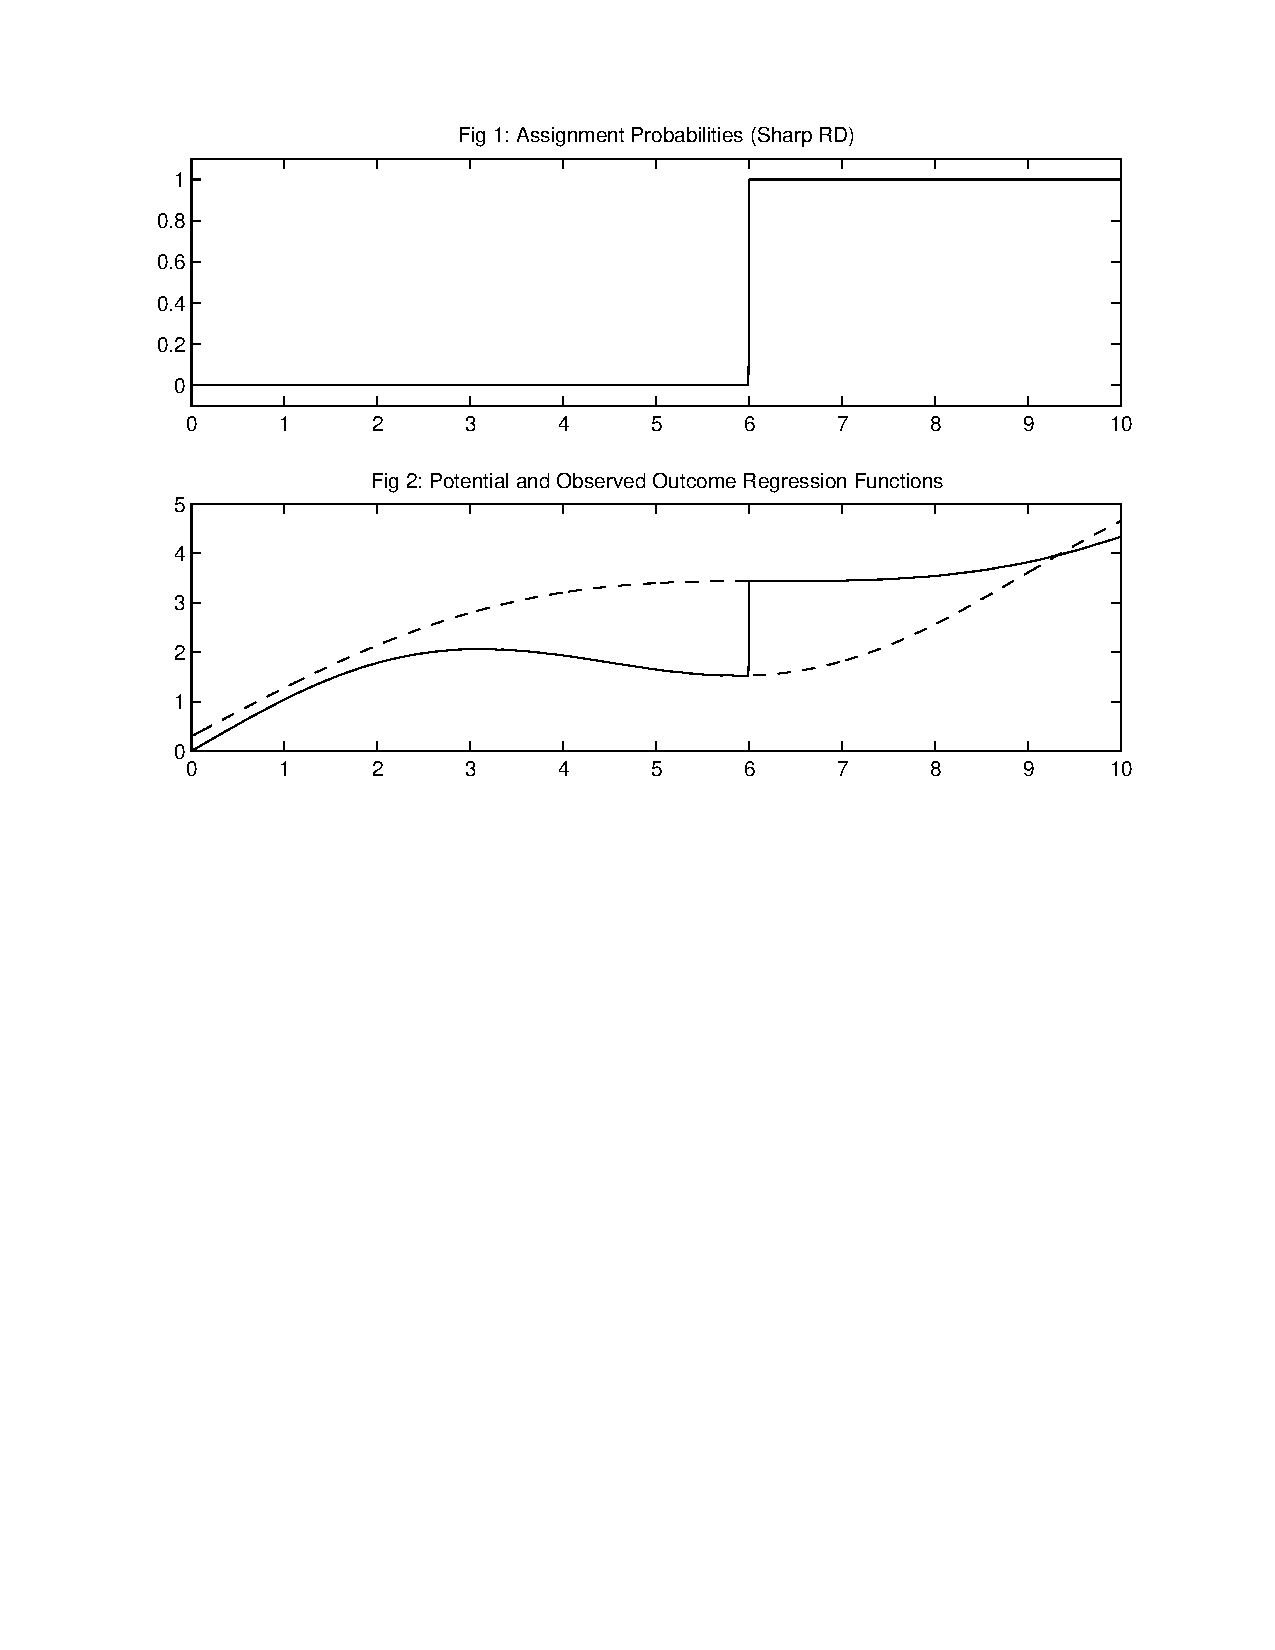
\includegraphics[scale=.60]{graphs/imbens_lemieux_fig1.pdf}
\end{figure}
\end{center}
 }

  \frame{ \frametitle{Fuzzy design}
\begin{center}
\begin{figure}[t]
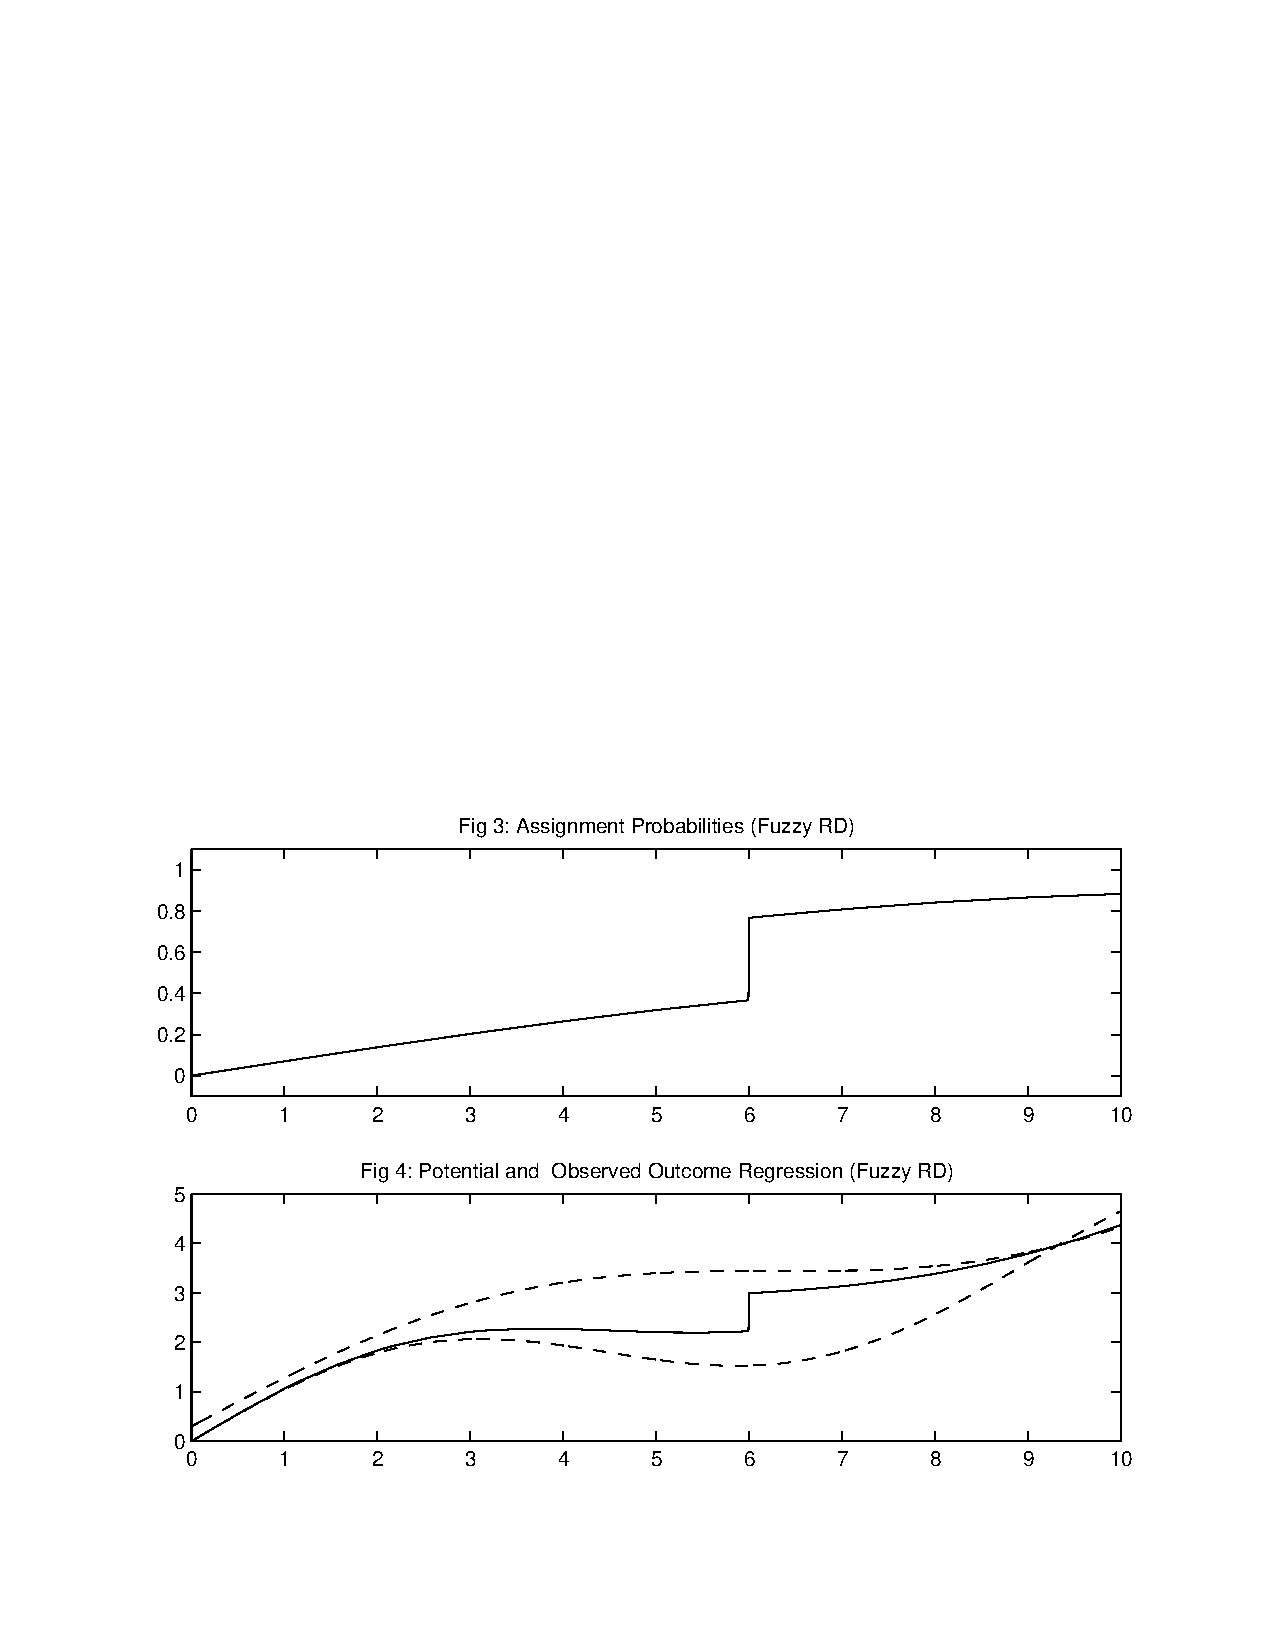
\includegraphics[scale=.60]{graphs/imbens_lemieux_fig2.pdf}
\end{figure}
\end{center}
 }



 \frame{ \frametitle{Notes}

Selection on observables:
\begin{equation*}
    ( Y_{1i},  Y_{0i}) \perp  D_i| z_i
\end{equation*}
holds trivially. In the sharp design there is no variation in $D_i$ conditional on $z_i$.

%"matching on a single variable"

\bigskip
But there is \textbf{zero overlap} with respect to $z$.

 }

  \frame{ \frametitle{Identification Assumptions}

\begin{enumerate}
  \item[RD.1] No difference in the outcome for those close to the cutoff in the absence of treatment. $E(Y_{0i}|z_i=z)$ is continuous at $z_0$, $E(Y_{1i}|z_i=z)$ is continuous at $z_0$.

  \item[RD.2] No sorting based on anticipated gains from treatment near the cutoff $E(x_{i}|z_i=z)$ is continuous at $z_0$.
\end{enumerate}
%These assumptions have testable implications!
 }


   \frame{ \frametitle{Identification of the treatment effect}

sharp design
\begin{equation*}
      \hat{\rho}_{s}= \underset{z \downarrow z_0}{lim} E(Y_i|z_i=z) -\underset{z\uparrow z_0}{lim} E(Y_i|z_i=z)
\end{equation*}

fuzzy design
\begin{equation*}
      \hat{\rho}_{f}= \frac{\underset{z \downarrow z_0}{lim} E(Y_i|z_i=z) -\underset{z\uparrow z_0}{lim} E(Y_i|z_i=z)}
     {\underset{z \downarrow z_0}{lim} E(D_i|z_i=z) -\underset{z\uparrow z_0}{lim} E(D_i|z_i=z)}
\end{equation*}
Notes:
\begin{itemize}
  \item We identify a \emph{local} treatment effect around the discontinuity
  \item Limited external validity, but strong internal validity of the result.
  \item The fuzzy RD estimator can be interpreted as an IV estimator (compare to Wald estimator)
\end{itemize}
 }


   \frame{ \frametitle{Estimation of the treatment effect}

\textbf{1. Graphical analysis}: Important part of any RD analysis!

\begin{itemize}
\item Group the data in bins with similar values of $z_i$  to the left and right of $z=z_0$.
\item  Plot mean \emph{outcomes} $Y_i$ in each bin  against $z$.
  \item Is there a jump in $Y$ at $z=z_0$?
  \item Are there jumps in mean outcomes at other values of $z \neq z_0$?
    \item First stage: Plot mean values of  $D_i$ in each bin against $z$, sharp or fuzzy design?
   \item  Testable assumptions: Plot mean values of \emph{covariates} $X_i$ in each bin.
   \item  Distribution of $z$: Plot the number of observations in each bin.
   \end{itemize}
 }
 
    \frame{ \frametitle{Estimation of the treatment effect}

\textbf{2. Regression analysis }
Local linear regression at the boundary, only use observations with values of $z$ close to the discontinuity
\begin{equation*}
      Y_i= \alpha +  \rho D_i +  \fmbeta \mb{z}_i + \varepsilon_i
\end{equation*}

Include more observations and control for flexible functions in $z$ to the left and right of $z=Z_0$
\begin{equation*}
      Y_i= \alpha +  \rho D_i + f_1(z_i - z_0) + D_i * f_2(z_i - z_0) + \fmbeta \mb{x}_i + \varepsilon_i
\end{equation*}
\begin{itemize}
  \item  $f_1$ and $f_2$ are polynomials in $(z-z_0)$
  \item $\delta$ measures the jump in $y$ at $z=z_0$
\end{itemize}

 }



   \frame{ \frametitle{Applications: Sharp Regression Discontinuity}
\begin{itemize}
  \item  Americans over 21 can drink legally
  \item American college presidents have lobbied to return the Minimum Legal Drinking Age (MLDA) at 18
  \item Theory (Amethyst Initiative): legal drinking at 18 avoids binge drinking contrasting the view  that the age-21 MLDA  reduces youth access to alcohol, preventing some harm
\end{itemize}
 }
 
 
 \frame{ \frametitle{}
\begin{center}
\begin{figure}[t]
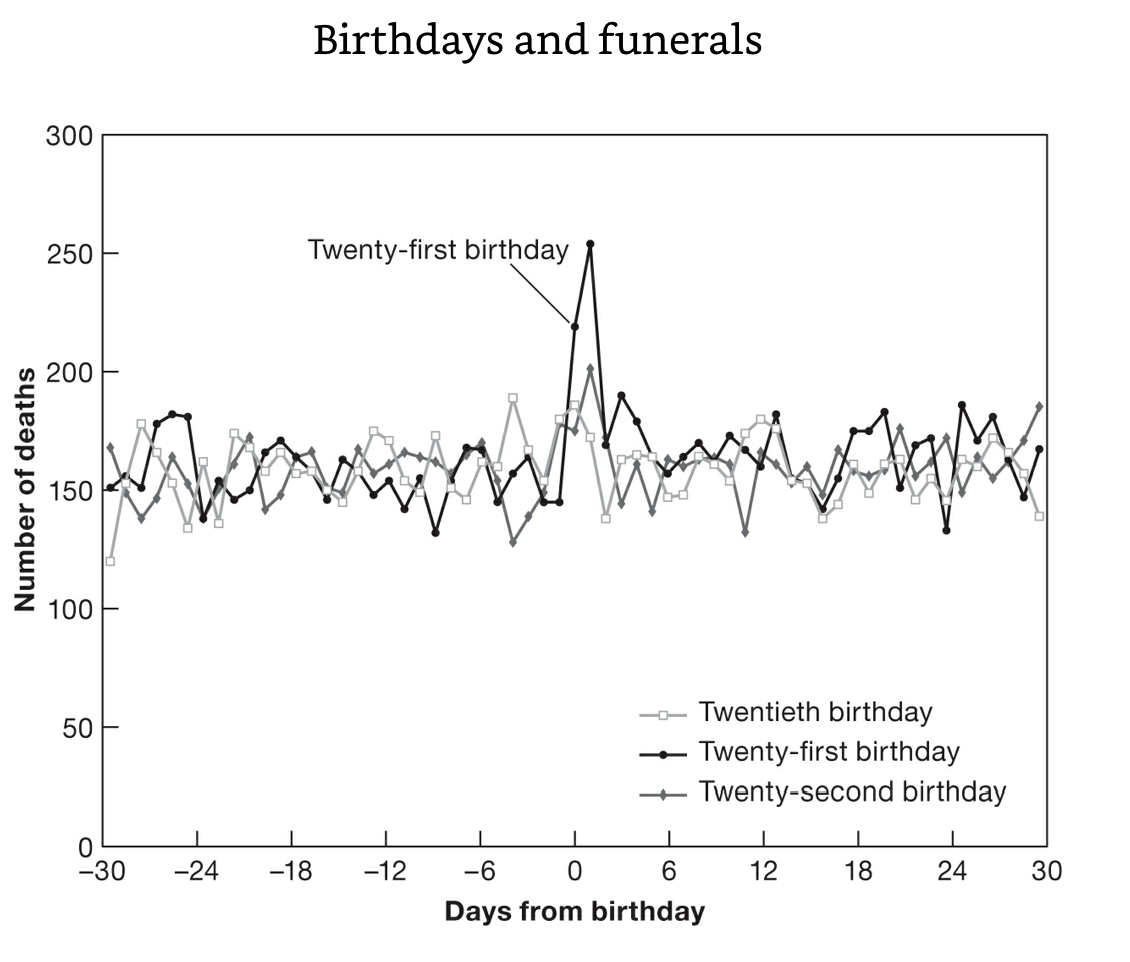
\includegraphics[scale=.50]{graphs/birthdays_funerals.png}
\end{figure}
\end{center}
 }
 
  \frame{ \frametitle{Minimum Drinking Age and Mortality Effects}
\begin{center}
\begin{figure}[t]
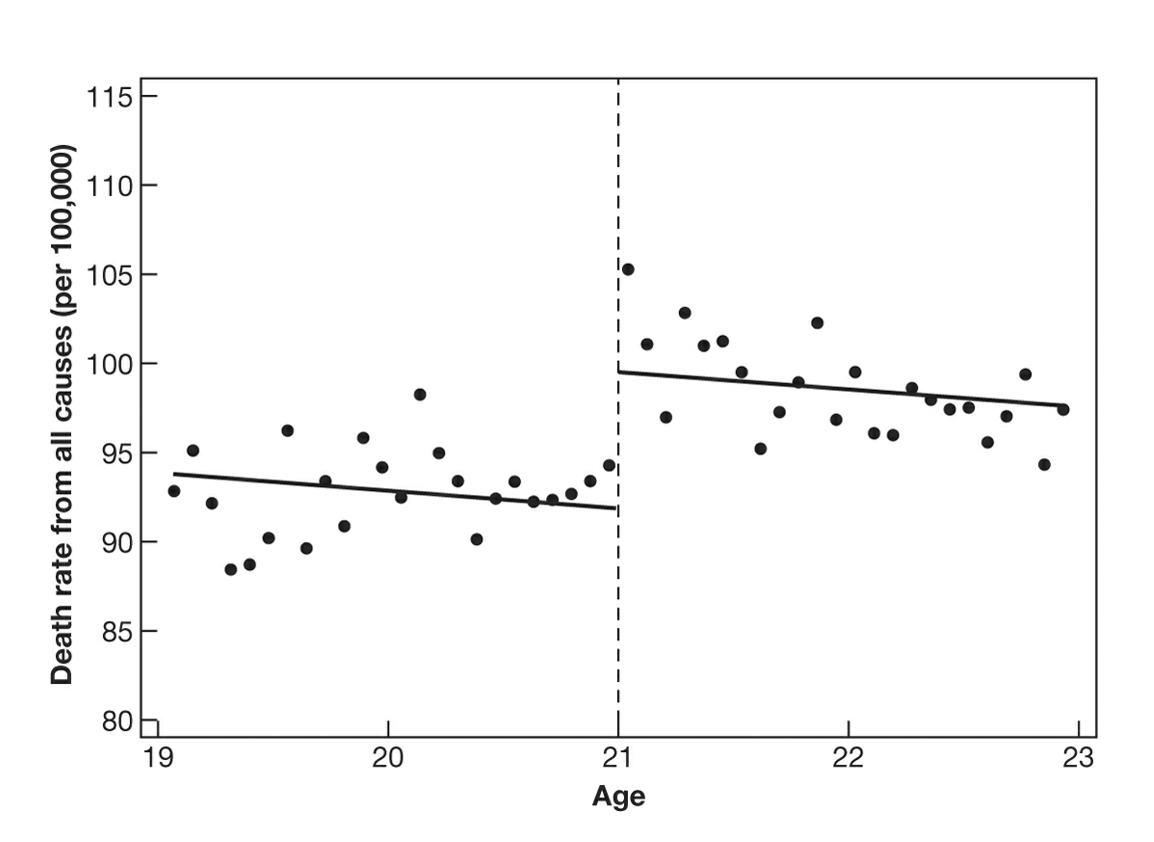
\includegraphics[scale=.50]{graphs/death_rate_year.png}
\end{figure}
\end{center}
 }
 
 \frame{ \frametitle{Minimum Drinking Age and Mortality Effects}
 $D_a$ is a deterministic function of $age$. Age is the running variable. MLDA is a sharp function of age
\begin{equation*}
    D_a =\left\{ \begin{array}{cc}
       1 & a \geq 21 \\
       0 & a < 21
     \end{array}
     \right.
\end{equation*}
\begin{itemize}

\item Treatment status is a deterministic function of $a$. Once we know $a$, we know  $D_a$
\item Treatment status is a discontinuous function of a, because no matter how close a gets to the cutoff, $D_a$ remains unchanged until the cutoff is reached.
\end{itemize}
}


 
    \frame{ \frametitle{Estimation of the treatment effect}

%Local linear regression at the boundary, only use observations with values of close to the discontinuity
\begin{equation*}
      M_a= \alpha +  \rho D_a + \gamma a  + \varepsilon_a
\end{equation*}
\begin{itemize}

\item where  $M_a$ is mortality in month $a$ defined as 30 day interval
\item RD tools aren't guaranteed to produce reliable causal estimates.
\begin{itemize}
\item Get as close to the cutoff as possible
\item Model nonlinearities directly as polynomial functions of the running variable on both sides of the discontinuity (no need to be the same degree of polynomial on both sides)
\end{itemize}
\end{itemize}
 } 
 
 
 
   \frame{ \frametitle{Three cases}
\begin{center}
\begin{figure}[t]
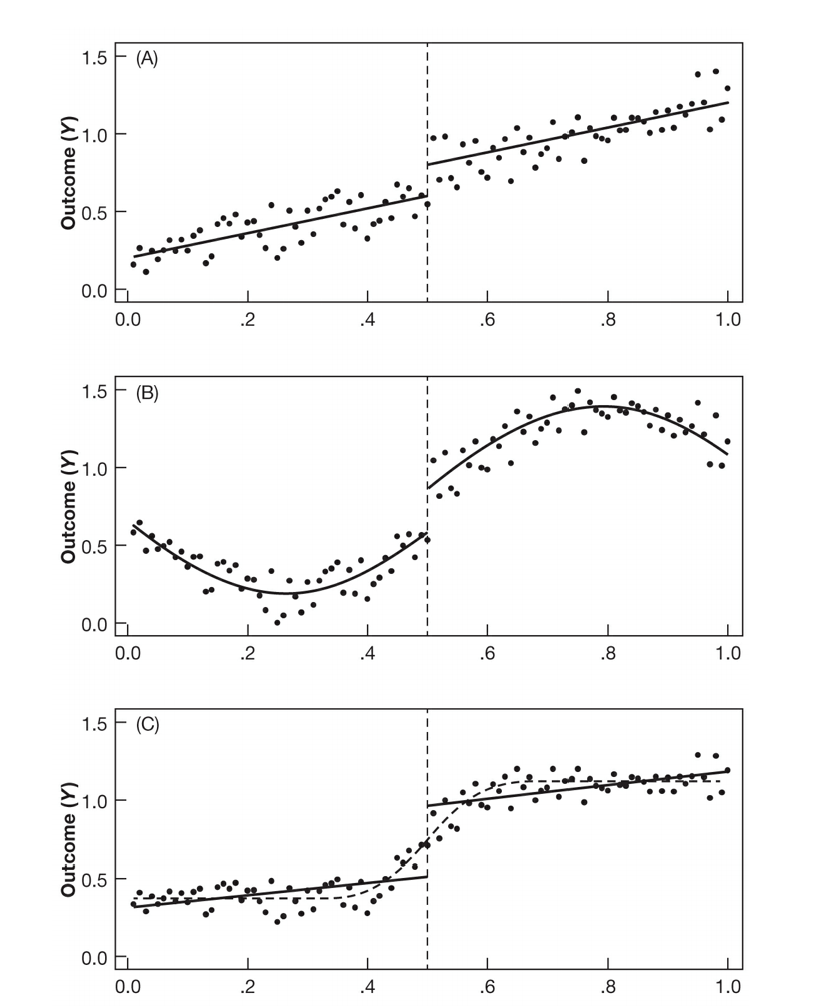
\includegraphics[scale=.40]{graphs/RD_three_cases.png}
\end{figure}
$z_i$
\end{center}
 }
 
    \frame{ \frametitle{What polynomial degree?}
\begin{itemize}

\item  Gelman and Imbens (2018) reccomend polynomials up to a quadratic to avoid the problem of overfitting. Usually, researchers report estimates with various degrees.

\item To make the model with interactions easier to interpret, we center the running variable by subtracting the cutoff
\begin{equation*}
\begin{aligned}
      M_a&=& \alpha +  \rho D_a+ \gamma_1 (a-21) + \gamma_2 (a-21)^2 +\\
      & & \delta_1[ D_a (a-21)] + \delta_2[ D_a  (a-21)^2 ] + \varepsilon_a
\end{aligned}
\end{equation*}
%\item treatment effect away from the cutoff is $\rho+\delta_1 (a-21) + \delta_2  (a-21)^2  $
\end{itemize}

 } 
 
 
   \frame{ \frametitle{}
\begin{center}
\begin{figure}[t]
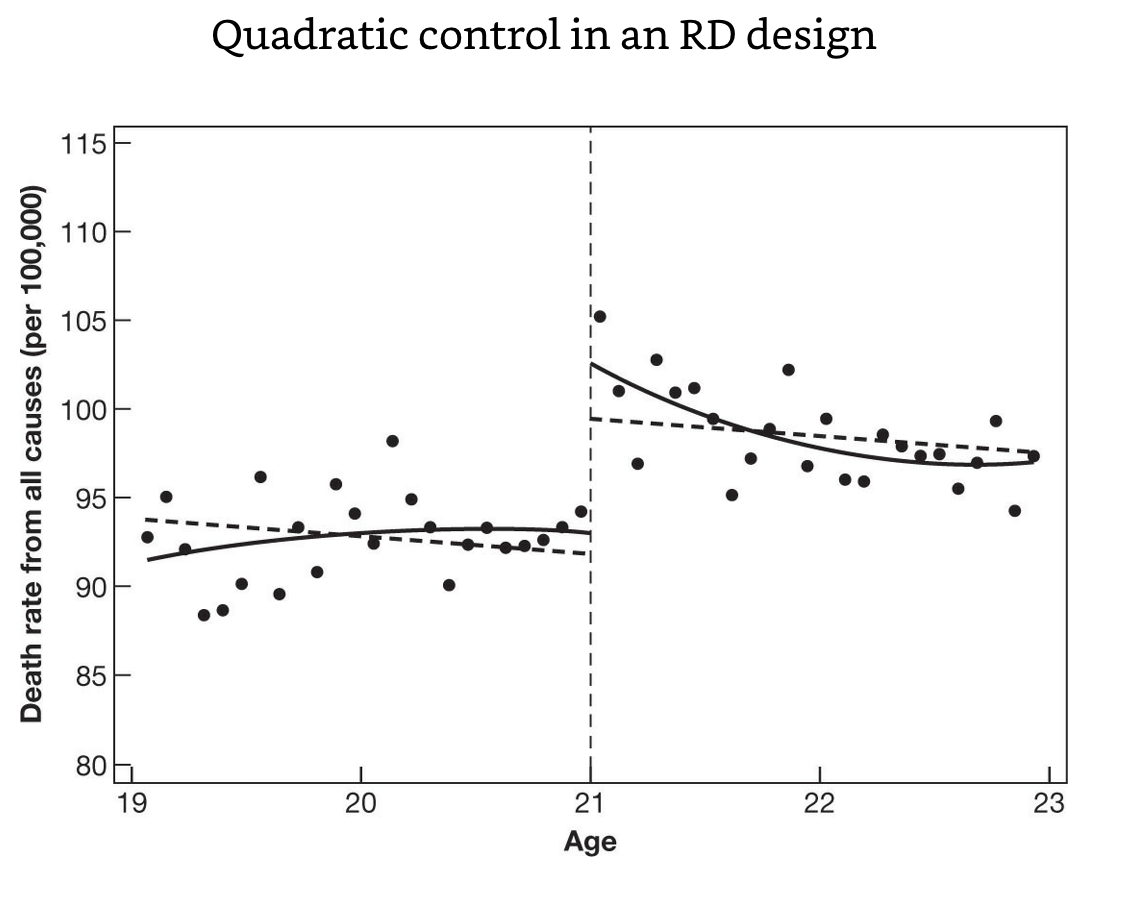
\includegraphics[scale=.50]{graphs/death_rate_quadratic.png}
\end{figure}
\end{center}
 }
 
    \frame{ \frametitle{Covariate Balance}
\begin{center}
\begin{figure}[t]
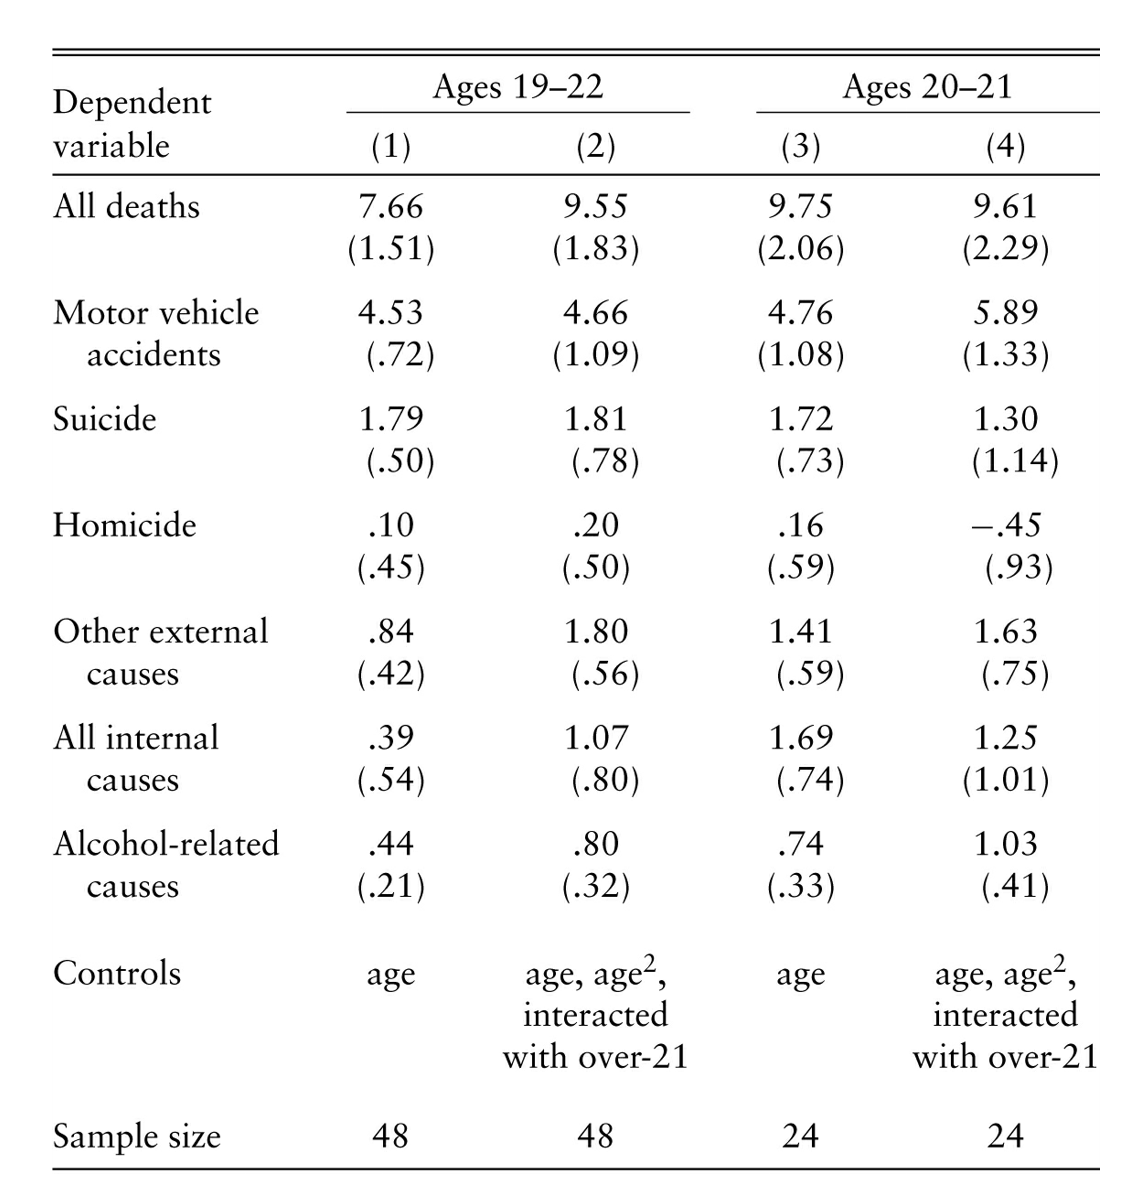
\includegraphics[scale=.40]{graphs/deaths_table.png}
\end{figure}
\end{center}
 } 
    \frame{ \frametitle{}
\begin{center}
\begin{figure}[t]
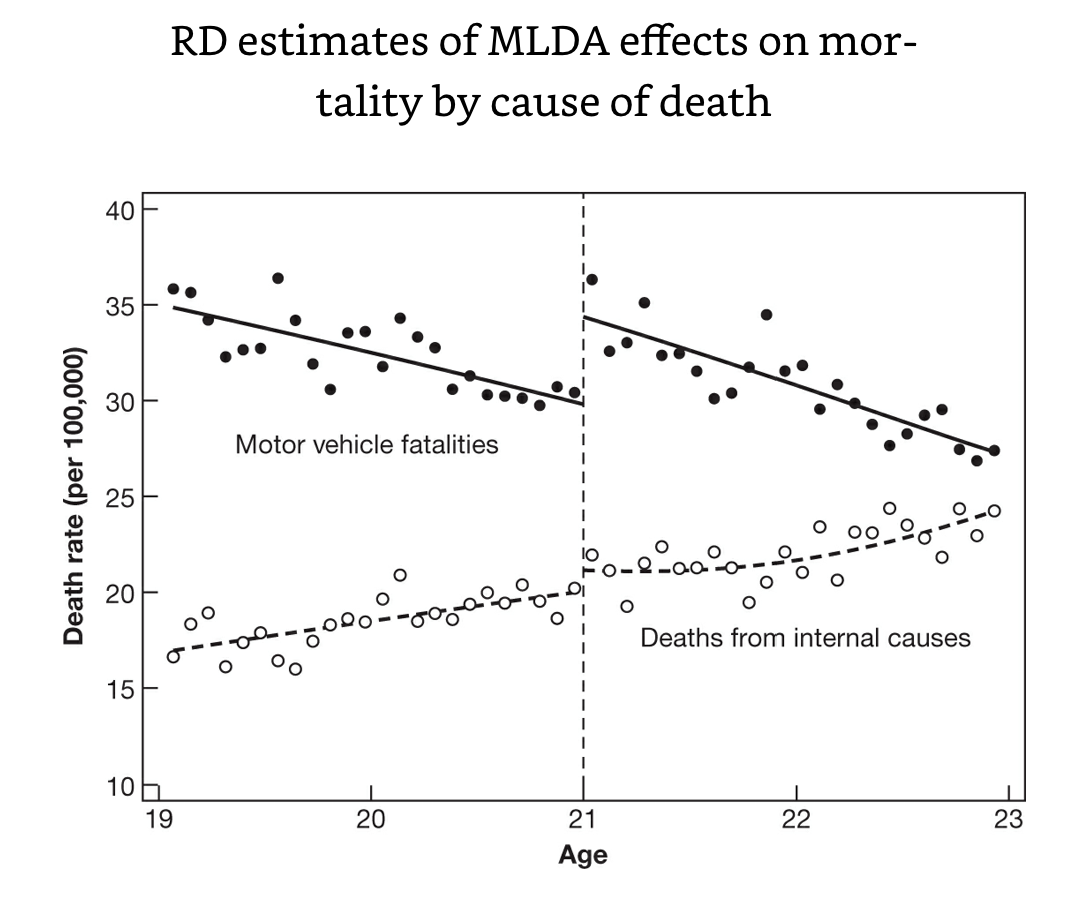
\includegraphics[scale=.50]{graphs/by_death_cause.png}
\end{figure}
\end{center}
 }
 
    \frame{ \frametitle{How close to the boundary?}
\begin{itemize}
\item As close as possible
\item Drawback:  few observations left. This causes the resulting estimates are likely to be too imprecise to be useful.

\item Solution:  Non-parametric RD

\item To make the model with interactions easier to interpret, we center the running variable by subtracting the cutoff
\begin{equation*}
\begin{aligned}
      M_a&=& \alpha +  \rho D_a+ \gamma a+  \varepsilon_a
\end{aligned}
\end{equation*}
\item in a sample such that: $a_0 -b \leq a  \leq a_0 +b  $
\item $b  $ is the bandwidth which is a function of sampling size
\item Theoretical econometricians have proposed strategies for making such bias-variance trade-offs efficiently. The bandwidth selection algorithm is not completely data-dependent and requires researchers to choose certain parameters.

\end{itemize}

 } 
 

 \frame{ \frametitle{Local linear nonparametric regression}
\begin{itemize}

\item Kernel regression as a weighted regression restricted to a window (bandwidth)
\item The kernel provides the weights to that regression. A rectangular kernel would give the same result as taking
$E[Y]$ at a given bin on $z$. The triangular kernel gives more importance
to the observations closest to the center.

\begin{equation*}
(\hat{\alpha}, \hat{\rho}) =\underset{\alpha, \rho }{argmin}  \sum_{i}^{n} (Y_i - \alpha -  \rho  (z_i-z_0))^2 K(\frac{z_i-z_0}{h})  \mathbbm{1}(z_i > z_0)
\end{equation*}



\end{itemize}

 }

 
 
 
 \frame{ \frametitle{RD recommendation}
\begin{itemize}
\item Hahn, Jinyong, Petra Todd, and Wilbert Van der Klaauw. "Identification and estimation of treatment effects with a regression-discontinuity design." Econometrica 69.1 (2001): 201-209.
  \item Imbens, Guido W. and Thomas Lemieux (2008) "Regression Discontinuity Designs: A Guide to Practice" Journal of Econometrics, 142, 615-635.
\item Gelman, Andrew, and Guido Imbens. "Why high-order polynomials should not be used in regression discontinuity designs." Journal of Business \& Economic Statistics (2018): 1-10.

\end{itemize}
}
\end{document}






